\begin{figure}[p]
  \centering
  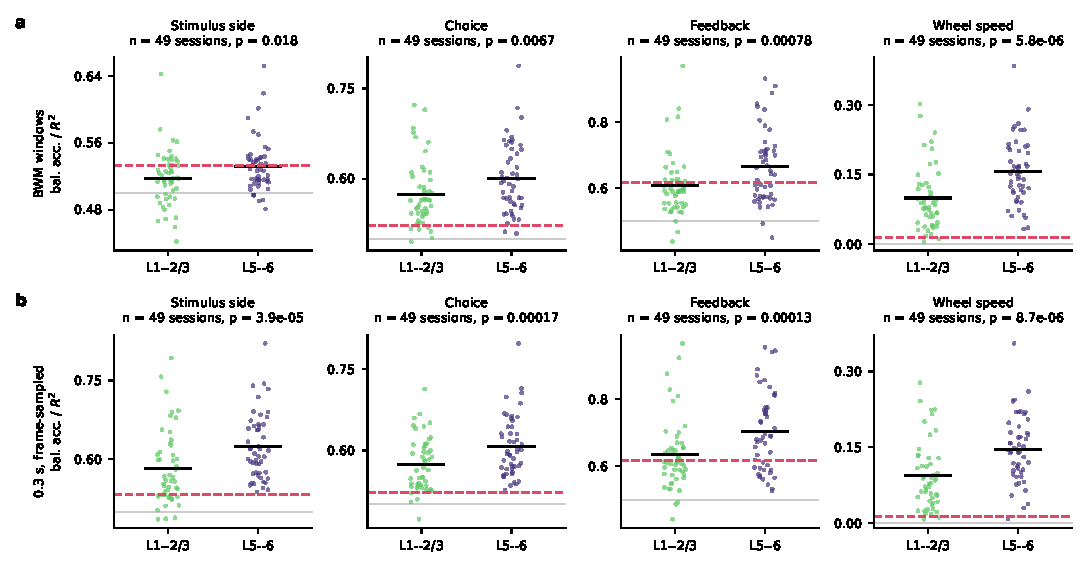
\includegraphics[width=7.00in,height=0.78\textheight,keepaspectratio]{si/si_layers_panels.pdf}
  \caption{Recording depth. Mesoscope neurons lie in L1--2/3 (by region label), while most BWM isocortex units lie in L5--6. Here decoders use 10 randomly drawn neurons of one layer group per session, ignoring spatial bins (mean of 10 draws), so both groups come from the same sessions. \textbf{a} BWM units with the BWM windows: decoding from 10 superficial (L1--2/3) vs 10 deep (L5--6) units of the same session (dots: sessions with $\geq$10 units in both groups; bars: means; Wilcoxon signed-rank test). Dashed line: mesoscope, 10 neurons per session. \textbf{b} Same with the 0.3\,s windows and frame sampling, the BWM version closest to how the mesoscope measures activity.}
  \label{fig:si_layers}
\end{figure}
